\section{Tarjeta}
Este trabajo, se separa en dos partes: software y hardware. Para el hardware se realizara una tarjeta la cual hemos nombrado SAM9-MX. Existen tarjetas parecidas a la nuestra, sin embargo, cuentan con componentes que no usaremos en este trabajo terminal y a dem\'as de funciones que optimizaremos con nuestro diseño.\medskip

Para la primer entrega de este trabajo, en la parte del hardware se presentar\'a: \medskip 
\begin{itemize}

\item Especificaci\'on de las funciones de nuestra trajeta
\item Especificaci\'on de los componentes de nuestra tarjeta
\item Diagrama de bloques de la SAM9-MX
\item Diagrama esquem\'atico de la SAM9-MX

\end{itemize}

\subsection{Funciones deseadas}

Para cumplir con los objetivos de este proyecto es deseable que el dise\~no de la tarjeta pueda ser utilizado para construir posteriormente un dispositivo m\'oviles, que adem\'as de manejar video en dos dimensiones, pueda utilizar una variedad de dispositivos externos como:

\begin{itemize}

\item Internet inal\'ambrico por medio de WiFi
\item Video en una pantalla LCD
\item Dispositivos de Entrada y Salida

\end{itemize}

Para ser usada como plataforma de desarrollo es necesario ser capaces de subir c\'odigo a la tarjeta de una manera sencilla los nuevos programas y cambios que desarrollemos.

Otro punto importante a tomar en cuenta es la salida de video, para ello hay que tomar en cuenta que se deben de poder guardar imagenes en una memoria de alta capacidad y poder trabajarlas en una memoria de mejor velocidad.

Es por ello que se han definido las siguientes capacidades importantes de la tarjeta:

\begin{itemize}

\item Reguladores de Voltaje a 3.3 volts.
\item Interfaz USB para f\'acil acceso a la computadora.
\item Interfaz con dispositivos de almacenamiento externos.
\item Interfaz para depurar y programaci\'on código.
\item Capacidad de conectar dispositivos de memoria externa.

\end{itemize}

Los dispositivos que se han seleccionado para cumplir con esta especificaci\'on se detallan en la subsecci\'on siguiente.

\subsection{Componentes}


Tabla de componentes de SAM9-MX

Para realizar la tarjeta claro esta, debemos tener una lista de materiales a utilizar, la cual esta descrita a continuaci\'on:\medskip

\textbf{Resistencias}

\begin{center}
\begin{tabular}{|c|c|c|c|}
\hline
\hline
\normalsize valor & \normalsize cantidad & \normalsize valor & \normalsize cantidad\\
\hline
\normalsize 1K & \normalsize 14 & \normalsize 470K & \normalsize 10\\
\hline
\normalsize 33K & \normalsize 10 & \normalsize 100K & \normalsize 6\\
\hline
\normalsize 100 & \normalsize 6 & \normalsize 10K & \normalsize 5\\
\hline
\normalsize 4.7K & \normalsize 5 & \normalsize 47 & \normalsize 4\\
\hline
\normalsize 39 & \normalsize 4 & \normalsize 3.3K & \normalsize 2\\
\hline
\normalsize 560 & \normalsize 2 & \normalsize 330 & \normalsize 2\\
\hline
\normalsize 1.5M & \normalsize 1 & \normalsize 22K & \normalsize 1\\
\hline
\normalsize 220 & \normalsize 1 & \normalsize  & \normalsize \\
\hline
\end{tabular}
\end{center}

\textbf{Capacitores}

\begin{center}
\begin{tabular}{|c|c|c|c|}
\hline
\hline
\normalsize valor & \normalsize cantidad & \normalsize valor & \normalsize cantidad\\
\hline
\normalsize 100nF & \normalsize 49 & \normalsize 10uF & \normalsize 9\\
\hline
\normalsize 1nF & \normalsize 4 & \normalsize 15pF & \normalsize 3\\
\hline
\normalsize 10pF & \normalsize 3 & \normalsize 47uF & \normalsize 3\\
\hline
\normalsize 10nF & \normalsize 2 & \normalsize 100uF & \normalsize 2\\
\hline
\normalsize 20pF & \normalsize 2 & \normalsize 1uF & \normalsize 2\\
\hline
\normalsize 33pF & \normalsize 1 & \normalsize 0.1uF & \normalsize 1\\
\hline
\normalsize MFR110 & \normalsize 1 & \normalsize MFR030 & \normalsize 1\\
\hline
\end{tabular}
\end{center}

\textbf{Bobinas}

\begin{center}
\begin{tabular}{|c|c|}
\hline
\hline
\normalsize valor & \normalsize cantidad\\
\hline
\normalsize 470nH & \normalsize 2\\
\hline
\normalsize FB0805 & \normalsize 1\\
\hline
\normalsize FB1206 & \normalsize 1\\
\hline
\end{tabular}
\end{center}

\textbf{Diodos}

\begin{center}
\begin{tabular}{|c|c|}
\hline
\hline
\normalsize valor & \normalsize cantidad\\
\hline
\normalsize BAT54C & \normalsize 1\\
\hline
\normalsize 1,5KE6 8CA & \normalsize 1\\
\hline
\end{tabular}
\end{center}

\textbf{LED}

\begin{center}
\begin{tabular}{|c|c|}
\hline
\hline
\normalsize valor & \normalsize cantidad\\
\hline
\normalsize Rojo & \normalsize 3\\
\hline
\normalsize Verde & \normalsize 2\\
\hline
\normalsize Amarillo & \normalsize 2\\
\hline
\end{tabular}
\end{center}

\textbf{Relojes}

\begin{center}
\begin{tabular}{|c|c|}
\hline
\hline
\normalsize valor & \normalsize cantidad\\
\hline
\normalsize 32.768kHz & \normalsize 1\\
\hline
\normalsize 18.324MHz & \normalsize 1\\
\hline
\end{tabular}
\end{center}

\textbf{USB}

\begin{center}
\begin{tabular}{|c|c|}
\hline
\hline
\normalsize valor & \normalsize cantidad\\
\hline
\normalsize USB Device & \normalsize 2\\
\hline
\normalsize USB Host & \normalsize 1\\
\hline
\end{tabular}
\end{center}

\textbf{Microcontrolador AT91SAM9260}\medskip

El AT91SAM9260 es el primer miembro de la familia de microcontroladores ARM9, comparte el mismo modelo de programación que los controladores ARM7 y permite la migración directa entre controladores basados en diferentes cores de ARM.  Soporta operaciones deterministas y de tiempo real, ofrece funciones de supervisación y tiene soporte de otras compañías comparada con los otros controladores de 8-bits.\medskip \cite{at91}

El AT91SAM9260 esta basado en el procesador ARM926EJ-S, cuenta con 8K byte de instrucciones y 8K de cache de datos. Opera a 210 MIPS con un reloj de 190MHZ. Contiene 8K bytes de SRAM y 32K bytes de ROM, aunado con un bus externo de interfaz con controladores de SDRAM y memorias estáticas incluyendo la memoria NAND Flash y CompactFlash.\medskip

Dentro de los puertos perif\'ericos se incluye USB Host y USB Device, puerto Ethernet, interfaz de sensor de imagen, interfaz MCI, controlador serial síncrono, USARTs, Interfaz SPI, 3 canales de 16 bits de Time Counter TC, interfaz TWI, 4 canales ADC de 10 bits. 3 puertos de 32 bits cada uno para entradas y salidas, canales perif\'ericos DMA para maximizar el paso de los datos entre las interfaces.\medskip

El AT91SAM9260 cuenta con un sistema de control completo que incluye reset, interruptor de apagado, reloj, AIC, DBGU, temporizador de intervalo periódico, temporizador watchdog y de tiempo real.\medskip
 
Soporta Linux y Windows CE. Ha sido desarrollado para aplicaciones de procesamiento de im\'agenes. Tales como terminales de punto de venta, c\'amaras basadas en Ethernet y decodificadores de barras.\medskip

\textbf{Memoria NAND MT29F8G08MADWC:DTR}\medskip

La MT29F8G08MADWC es una memoria NAND flash de 8GB. Esta memoria NAND incluye las caracter\'isticas est\'andar de todas las dem\'as NANd Flash de micron as\'i como una nueva caracter\'istica diseñada para mejorar el rendimiento del sistema.\medskip \cite{mt29}

La MT29F8G08MADWC usa un bus multiplexor de 8 bits para transferir datos, direcciones e instrucciones. Los 5 pins de comandos (CLE, ALE, CE, RE, WE) implementan el protocolo de interfaz del bus de comandos. Dos pines adicionales controlan la protecci\'on de escritura del hardware (WP) y el estado del monitor (R/B).\medskip

\textbf{Memoria Ram MT48LCG64M4A2P-75}\medskip

La SDRAM de 256Mb es un CMOS de alta velocidad. Esta configurada internamente con cuatro bancos DRAM con una interfaz s\'incrona integrada. Cada uno de los bancos esta organizado con 8,192 filas y 512 columnas.\medskip \cite{mt48}

Los accesos de la SDRAM son orientados a flujos, Los accesos empiezan con el registro del comando ACTIVE, despu\'es le sigue el comando READ o WRITE. Los bits de direcciones que coinciden con el comando ACTIVE son usados para seleccionar el banco y la fila a la que se quiere accesar (BA0, BA1 selecciona el banco; A0-A12 selecciona la fila) Los bits de direcciones que coinciden con los comandos READ y WRITE, son usados para seleccionar donde empezar\'a la columna de acceso.\medskip

La SDRAM de 256Mb usa arquitectura pipeline para logar la r\'apida velocidad de operaci\'on. Al precargar un banco mientras se accesa a uno de los otros 3 bancos esconder\'a los ciclos precargados y provee alta velocidad en operaciones aleatorias de acceso.\medskip

La SDRAM esta diseñada para operar en sistemas de memorias de 3.3V.\medskip

\textbf{Memoria Flash AT45DB16ID-SU}\medskip

La AT45DB161D-SU es una memoria Flash de 2.5volts a 2.7 volts ideal para aplicaciones de  almacenamiento de datos, voz digital e im\'agenes. Soporta la interfaz serial RapidS para aplicaciones que requieren operaciones de alta velocidad. La interfaz serial RapidS es compatible para frecuencias de hasta los 66MHz.\medskip \cite{at45}

Esta memoria esta organizada en 4,096 p\'aginas de 512 bytes o de 528 bytes cada una. As\'i mismo la memoria principal contiene dos buffers SRAM de 512 o 528 bytes cada uno. Los buffers permiten la recepci\'on de datos mientras la p\'agina en la memoria principal esta siendo reprogramada. \medskip

La memoria Flash utiliza la interaz serial RapidS para acceder secuencialmente a los datos, lo cual reduce la cantidad de pines activos que se deben tener para este proceso, incrementa la confiabilidad del sistema, minimiza el ruido, y disminuye el tamaño de los paquetes. Este dispositivo es usado de manera comercial en aplicaciones industriales donde la alta densidad, un n\'umero menor de pines activos, el bajo voltaje y la baja potencia son esenciales.\medskip

Para permitir la capacidad de reprogramaci\'on del sistema, la  AT45DB161D no requiere de altos voltajes para programarla. El dispositivo opera con una sola fuente de alimentaci\'on, 2.5V a 3.6V o 2.7V a 3.6V, para las operaciones de programaci\'on y de lectura. \medskip

\textbf{FT232RL}\medskip

El FT232RL es el m\'as reciente dispositivo de la familia FTDI USB UART. El FT232RL es una interfaz de usb a UART serial con reloj opcional generador de salidas y el nuevo FTDIChip-ID. As\'i mismo, contiene los bits bangs de interfaz en modos asincr\'onos y s\'incronos est\'an disponibles. El diseño USB a serial utilizando el FT232R se ha simplicado gracias a integrar la EEPROM externa, el reloj del circuito y los resistores USB dentro del dispositivo. \medskip \cite{ft232}

El FT232RL tiene dos nuevas funciones. El reloj interno se puede usar fuera del dispositivo para controlar un microcontrolador. Un n\'umero unico es impreso en el dispositivo durante la realizaci\'on del mismo el cual se lee por el USB, formando un chip de seguridad que se utilizar para proteger el software de ser copiado.\medskip

\subsection{Diagrama de bloques}

Una vez que ya se tiene bien claros cuales son los componentes a utilizar y las funciones que se quiere abarcar con nuestra tarjeta, se procede a realizar un diagrama de bloques.\medskip

El diagrama de bloques es la representaci\'on gr\'afica del funcionamiento interno de un sistema, que se hace mediante bloques y sus relaciones, y que, adem\'as, definen la organizaci\'on de todo el proceso interno, sus entradas y sus salidas.\medskip

En este diagrama de bloques se muestra a continuaci\'on como estan relacionados los distintos componentes, los m\'as relevantes, con el microcontrolador, se especifica cuantos son los pines que est\'an conectados con el micro para as\'i darnos una idea de la cantidad de pines que debe tener disponibles el AT91SAM9260.

\begin{figure}[H]
\centering
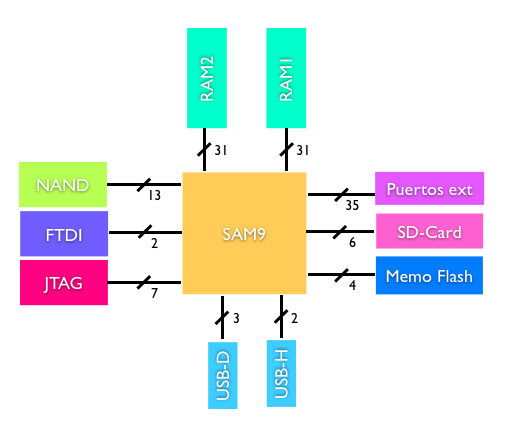
\includegraphics[scale=0.8]{diagrama_bloques}
\caption{Diagrama de bloques de SAM9-MX}\label{fig:diagrama_bloques}
\end{figure}

\subsection{Diagrama esquem\'atico}

El diagrama esquem\'atico es una representaci\'on pict\'orica de un circuito el\'ectrico. Muestra los diferentes componentes del circuito de manera simple y con pictogramas uniformes de acuerdo a normas, y las conexiones de poder y de señales entre los dispositivos. El arreglo de los componentes e interconexiones en el esquema generalmente no corresponde a sus ubicaciones f\'isicas en el dispositivo terminado.\medskip

El diagrama esquem\'atico que se muestra en la siguiente figura contiene todos los componentes de la tarjeta SAM9-MX juntos con todos sus pines. Se puede ver facilmente como estan conectados entre s\'i. De esta forma se tiene una idea de la organizaci\'on que se debe cuidar a la hora de hacer el PCB.\medskip

\begin{figure}[H]
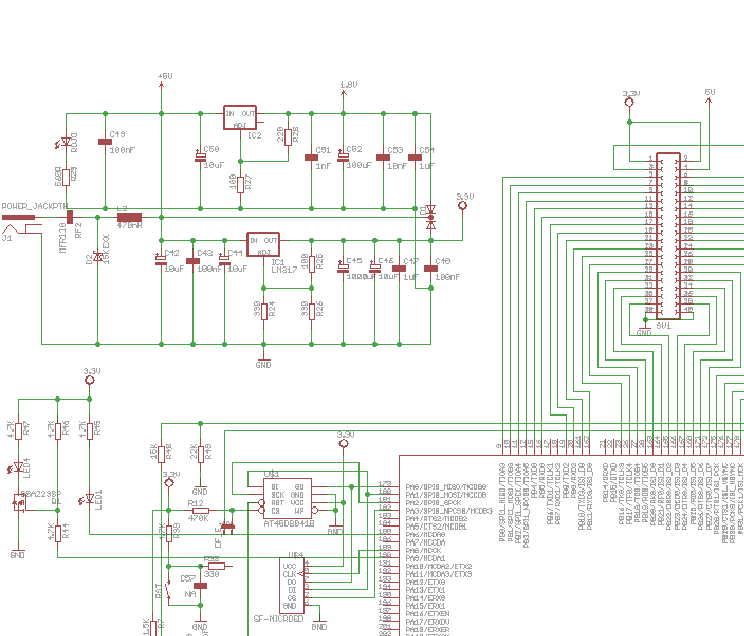
\includegraphics[scale=0.55]{samEsq1}
\caption{Diagrama esquematico parte 1 de 4 de SAM9-MX}\label{fig:samEsq1}
\end{figure}

En esta primera imagen se puede ver la parte de alimentaci\'on de la tarjeta, en la esquina superior izquierda, aqu\'i es donde se obtiene el voltaje que se necesita para alimentar a todos los componentes de la tarjeta los cuales en su mayor\'ia operan con 3.3V.\medskip

As\'i mismo se puede observar un espacio para puertos externos, esto es previniendo la posibilidad de que en un futuro se quieran conectar m\'as componentes de los que tiene esta tarjeta, y se pueden hacer en este espacio, que va directamente relacionado con los puertos B y C del micro.\medskip

Abajo, nos encontramos con dos componentes importantes, uno de ellos es la memoria Flash, cuyas caracter\'isticas fueron descritas anteriormente, \'esta est\'a conectada con algunos pines a nuestro micro, y tiene la posibilidad de deshabilitarla funci\'on que sirve en gran manera para nuestros prop\'ositos de programaci\'on.\medskip

Por \'ultimo, en esta parte del diagrama se puede ver la memoria SD Card, la cual decidimos fuera una micro SD, ya es un componente novedoso y f\'acil de usar para guardar o insertar datos a la tarjeta.\medskip

\begin{figure}[H]
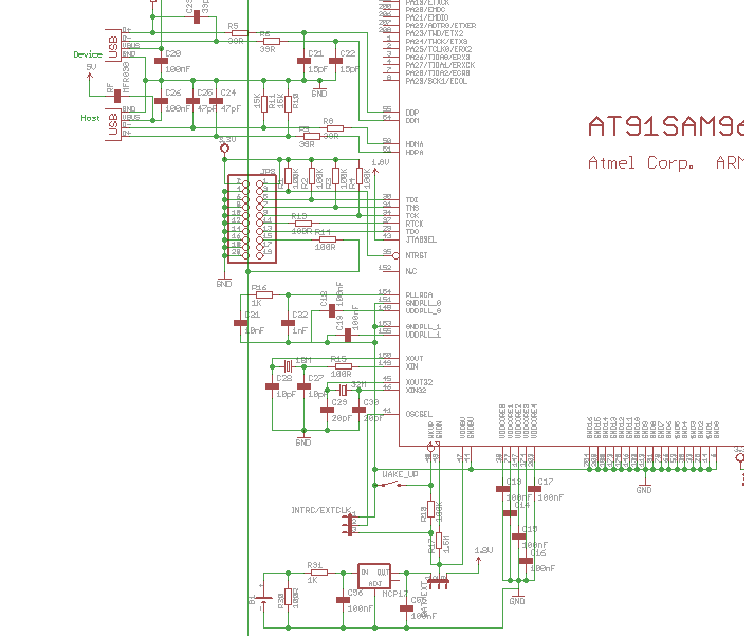
\includegraphics[scale=0.55]{samEsq2}
\caption{Diagrama esquematico parte 2 de 4 de SAM9-MX}\label{fig:samEsq2}
\end{figure}

En esta parte del diagrama de la tarjeta SAM9-MX, se pueden apreciar los dos puertos usb con los que cuenta, uno de ellos es un puerto USB Device el cual se puede comunicar con la computadora por medio un cable USB, y el otro puerto USB es Host, lo que nos permite directamente conectar nuestra memoria USB a la tarjeta,
estas son unas funciones innovadoras y faciles para el uso de nuestra tarjeta.\medskip

Otro componente importante es el JTAG, el cual nos sirve para programa y debuggear nuestra tarjeta, tambi\'en nos ayuda a saber los estados de los registros de la memoria, cuando se est\'a en tiempo de ejecuci\'on.\medskip

\begin{figure}[H]
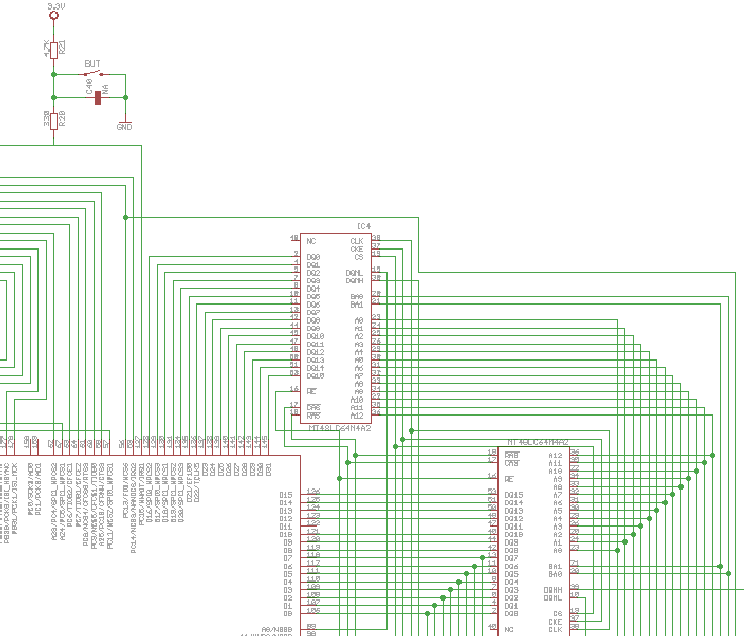
\includegraphics[scale=0.55]{samEsq3}
\caption{Diagrama esquematico parte 3 de 4 de SAM9-MX}\label{fig:samEsq3}
\end{figure}

Ahora podemos ver a las memorias RAM, nuestra tarjeta cuenta con dos de ellas para funcionamiento ya que en una se guarda la mitad alta de una direcci\'on de memoria mientras que en la otra se guarda la mitad baja de esa misma direcci\'on, las memorias estan conectadas a nuestro micro, por los pines de direcci\'on y los de datos.\medskip

\begin{figure}[H]
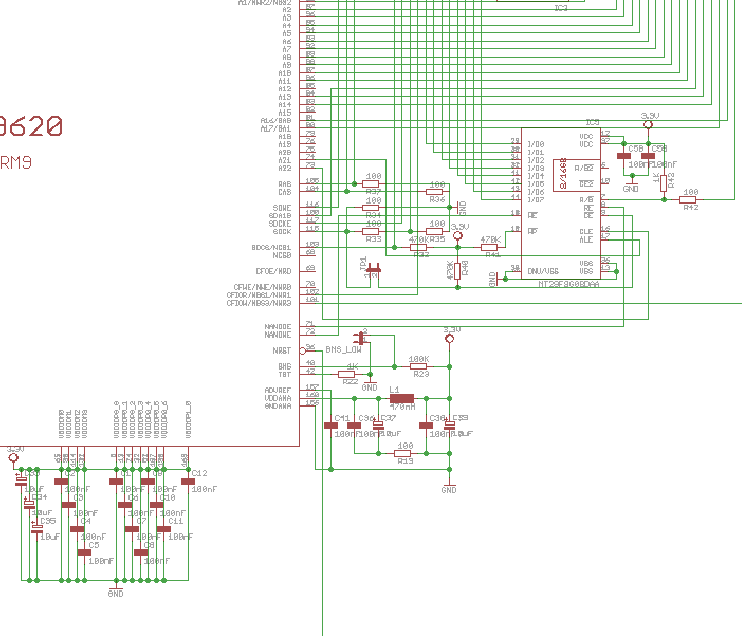
\includegraphics[scale=0.55]{samEsq4}
\caption{Diagrama esquematico parte 4 de 4 de SAM9-MX}\label{fig:samEsq4}
\end{figure}

Aqu\'i podemos ver a la memoria NAND Flash la cual puede ser deshabilitada o no para usarse en lugar de las memorias RAM, ya anteriormente descritas, por esa raz\'on comparten los pines del puerto D, de datos,  entre ellas, que est\'an conectados al micro.\medskip

\begin{figure}[H]
\centering
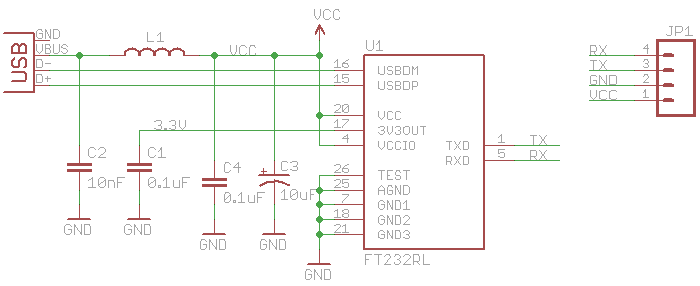
\includegraphics[scale=0.9]{ftdiEsquematico}
\caption{Diagrama esquematico del FTDI}\label{fig:ftdiEsquematico}
\end{figure}

Una de las mejoras que se quiere hacer para esta tarjeta es la de poner un FTDI en lugar del puerto serial, haciendo que la comunicaci\'on sea libre de ruido y as\'i mismo nos evitamos de molestos cables innecesarios, para esta entrega ya se tiene el diagrama esquem\'atico del FTDI que ser\'a posteriormente incluido en la tarjeta SAM9-MX.\medskip

